\documentclass[a4paper]{article}
\usepackage{hyperxmp}
\usepackage{titling}
\usepackage[colorlinks,linkcolor=blue]{hyperref}
\usepackage{graphicx}
\usepackage{fancyhdr}
\usepackage{a4wide}
\usepackage{xspace}
\usepackage{bbding}
\usepackage{dictsym}
\usepackage{lastpage}
\usepackage{tikz}

\makeatletter
\newcommand*{\rom}[1]{\expandafter\@slowromancap\romannumeral #1@\xspace}
\makeatother

\newcommand{\myhref}[2]{{\href{#1}{\textcolor{blue}{#2}}}}
\fancyhead[L]{\thetitle}
\fancyhead[R]{\it\thepage\ of \pageref{LastPage}}
\fancyfoot[C]{\centerline{\small \copyright\ \theauthor, 2013. This work is licensed under a \myhref{http://creativecommons.org/licenses/by-sa/3.0/}{Creative Commons Attribution-ShareAlike 3.0 Unported License.}}}
\pagestyle{fancy}

%% PDF meta-data
\hypersetup{%
pdftitle={Assigment 1 for the course on city design. Ideas and Forces That Have Shaped Your City},
pdfauthor={Vitaly Repin},
pdfcopyright={This work is licensed under a Creative Commons Attribution-ShareAlike 3.0 Unported License},
pdfsubject={Designing City},
pdfkeywords={design,city,map},
pdflicenseurl={http://creativecommons.org/licenses/by-sa/3.0/},
pdfcaptionwriter={Vitaly Repin},
pdfcontactcity={Espoo},
pdfcontactcountry={Finland},
pdfcontactemail={vitaly.repin@gmail.com},
pdflang={en}
}

%% City name
\newcommand{\mycity}{Espoo\xspace}
%% Author
\author{Vitaly Repin}
%% Title
\title{Ideas and Forces That Have Shaped My City: \emph{\mycity}}

\definecolor{myblue}{HTML}{0EBFE9}
%% Adapted from: http://tex.stackexchange.com/questions/7032/good-way-to-make-textcircled-numbers
%% Can be used only inzide tikzpicture environment
\newcommand{\circled}[2]{\node[shape=circle,draw,inner sep=2pt,fill=myblue] at (#1) {\textcolor{white}{#2}};}
%% Dtand-alone version of the command \circled
\newcommand{\circledd}[1]{\raisebox{-.18cm}{\begin{tikzpicture}\circled{0,0}{#1}\end{tikzpicture}}\xspace}

\date{October, 2013}

\begin{document}

\section{Introduction}
City of Espoo is the second largest city in Finland. Area of Espoo is $528\, km^2,$ population is approximately $250 000.$~\cite{espoofacts}.

Espoo differs from conventional Finnish city plans, which are formed around a single centre. Espoo consists of five city centres (each of which is the equivalent of a medium-sized Finnish city)
and two local centres~\cite{gov}.  One of these five city centers is ``Espoon Keskus'' (Espoo Centre), one of the local centers is Kauklahti. This paper is focused on Espoon Keskus and Kauklahti.

The following markers are used in the maps:
\begin{description}
\item[\circledd{1}] \myhref{http://www.espoo.fi/en-US/Housing_and_environment/Housing/City_centres/Kauklahti}{Kauklahti area.}
\item[\circledd{2}] \myhref{http://www.espoo.fi/en-US/Housing_and_environment/Housing/City_centres/Espoo_centre}{Espoon Keskus area.}
\item[\circledd{3}] Park on the border of Espoo and \myhref{http://www.hel.fi/hel2/irbc/kauniainen.html}{Kauniainen} (separate ``garden city'' of 8860 inhabitants surrounded by Espoo).
\item[\circledd{\CrossBoldOutline}] Espoo Cathedral. The oldest building in the city.
\item[\circledd{\dsrailways}] Espoo Railway Station.
\end{description}

%% Environment to draw maps
\newenvironment{mymap}[1]{%
\begin{tikzpicture}
%% Change scale size to suit your needs
\node[anchor=south west,inner sep=0] (image) at (0,0) {\includegraphics[keepaspectratio,width=\textwidth]{#1}};
\begin{scope}[x={(image.south east)},y={(image.north west)}]
}{
\end{scope}
\end{tikzpicture}
}

%% Page 1: Map of the city in IXX century
\section{Map of \mycity in \rom{19} century}

\begin{mymap}{map1}
\circled{0.1,0.3}{1}
\circled{0.44,0.48}{2}
\circled{0.75,0.56}{3}
\circled{0.42,0.57}{\CrossBoldOutline}
\end{mymap}
\centerline{Map of Espoo (Espoon keskus (city center) and Kauklahti areas) in 1855~\cite{espoo1855}.}
\medskip

The first inhabitants in the area arrived about 9,000 years ago.
The construction of the Espoo Cathedral (1480, \circledd{\CrossBoldOutline} in the map), the oldest preserved building in Espoo, marks the independence of Espoo.

The administrative center Espoon keskus has grown around the church and the Espoo railway station (built in 1903), but the municipality has retained a network-like structure of to the modern
day~\cite{wikip}.
\newpage

%% Page 2: Map of the city in the mid-20th century,
\section{Map of \mycity in the mid-\rom{20} century}
\begin{mymap}{map2}
\circled{0.14,0.33}{1}
\circled{0.6,0.6}{2}
\circled{0.88,0.73}{3}
\circled{.55,.63}{\dsrailways}
\circled{.51,.74}{\CrossBoldOutline}
\end{mymap}
\centerline{Map of Espoo (Espoon keskus (city center) and Kauklahti areas) in 1945~\cite{espoo1945}.}
\medskip

Espoo railway station (marked with \circledd{\dsrailways} in the map) was built in 1903.
\smallskip

Espoo started to grow rapidly in the 1940s and '50s. It quickly developed from a rural municipality into a fully-fledged industrial city, gaining city rights in 1972.
Due to its proximity to Helsinki, Espoo soon became popular amongst people working in the capital. In the fifty years from 1950 to 2000, the population of Espoo grew from 22,000 to 210,000.
The population growth is still continuing, but at a slower rate~\cite{wikip}.

\newpage

%% Page 3: Map of the city today (screenshot from http://www.openstreetmap.org/
\section{Map of \mycity in the year of 2013}
%% Change scale size to suit your needs
\begin{mymap}{map3}
\circled{0.05,0.22}{1}
\circled{0.63,0.54}{2}
\circled{0.9,0.7}{3}
\circled{0.56,0.67}{\CrossBoldOutline}
\circled{0.57,.56}{\dsrailways}
\end{mymap}
\centerline{Map of Espoo (Espoon keskus (city center) and Kauklahti areas) in 2013~\cite{espoo2013}.}
\medskip

Keh\"{a} III (national road 50) is an important highway in Southern Finland. It is the outermost of the three beltways in the Helsinki region, and the first one to be built.
The beginning was constructed between 1962 and 1965. The amount of traffic grew considerably over time and as a result the original intersections with
Helsinki's exit roads became dangerous. Therefore, all intersections with the city exits had been rebuilt as merging loops by the beginning of the 1970s.
The road has undergone almost continual modification and widening throughout its existence as traffic has increased in the region~\cite{keha3}.
\smallskip

Statistics for the 31 Aug, 2013~\cite{wikip}:

\begin{description}
\item[Population (Total)] $259,383$
\item[Rank] 2nd largest in Finland
\item[Density] $830.66/km^2 (2,151.4/mi^2)$
\end{description}

Kauklahti population is 6,191 (data for 2006)~\cite{wikip}.
\newpage

%% Page 4: Photographs
\newcommand{\desc}[2]{\raisebox{#1}{\parbox{.5\textwidth}{#2}}}
\section{Photographs of \mycity}
\begin{tabular}{lp{.5\textwidth}}
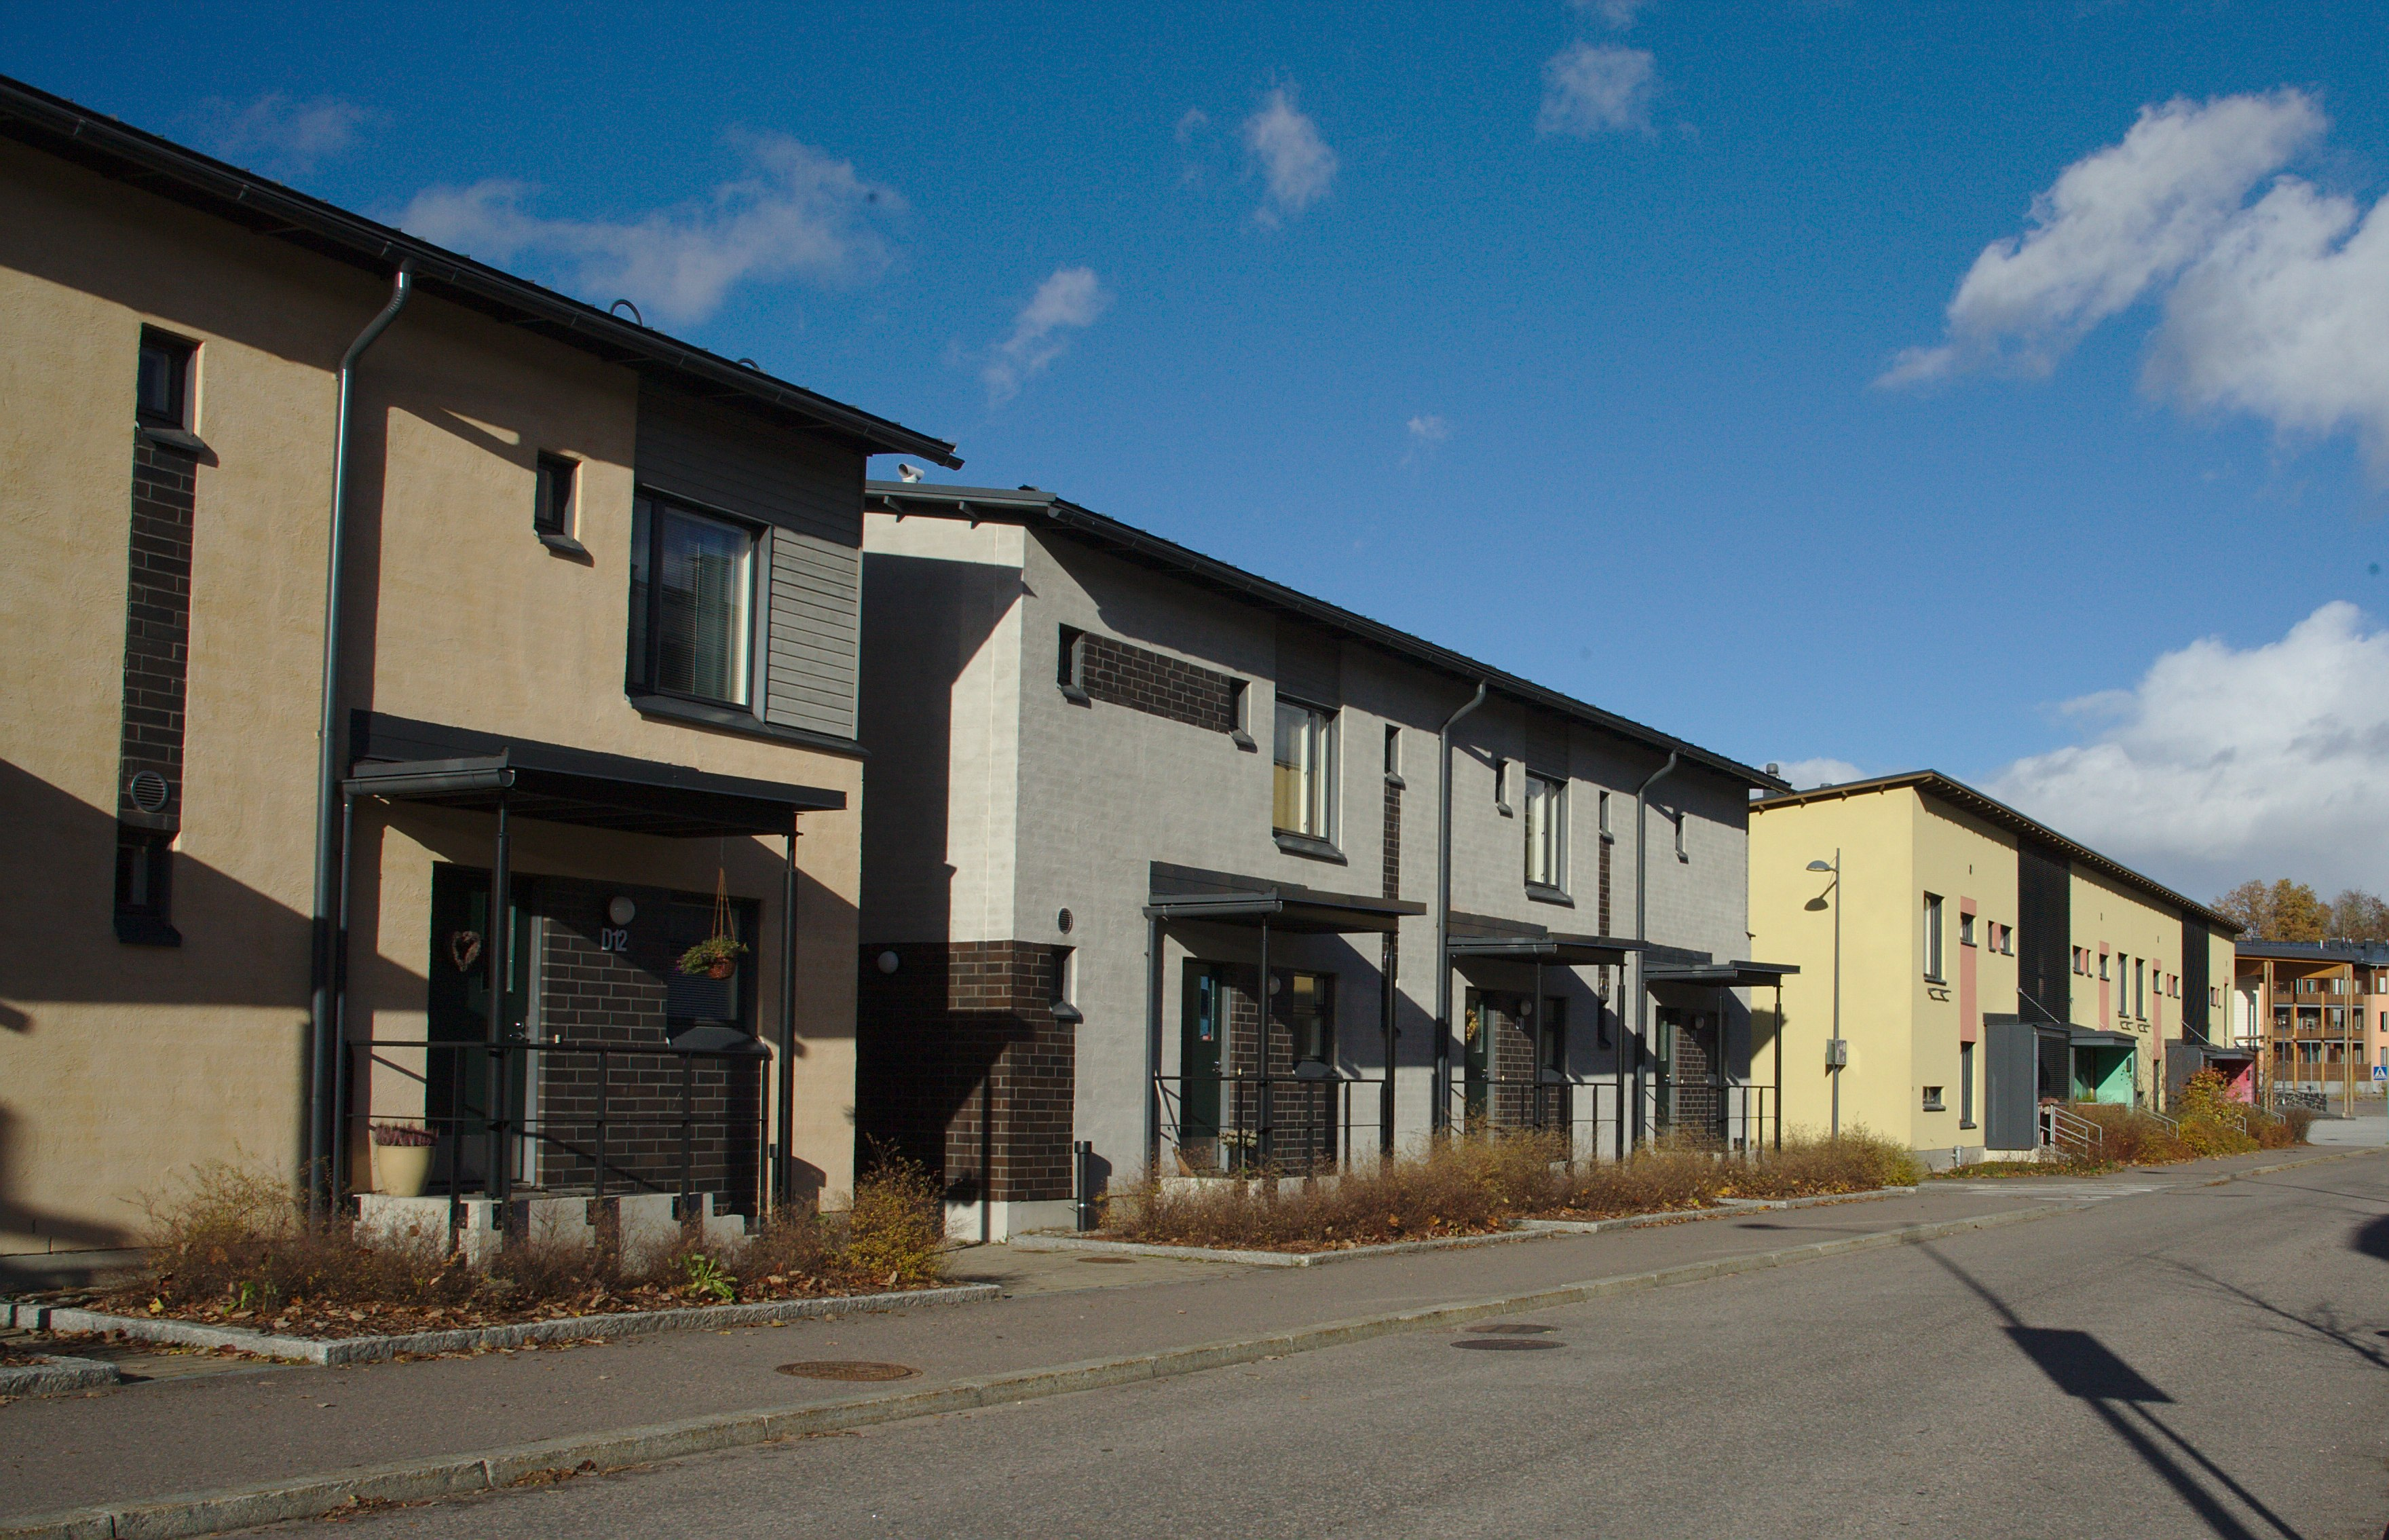
\includegraphics[keepaspectratio,width=.5\textwidth]{traditional} & \desc{4cm}{\circledd{1} Example of traditional city design in\\ Kauklahti.}\\[.2cm]
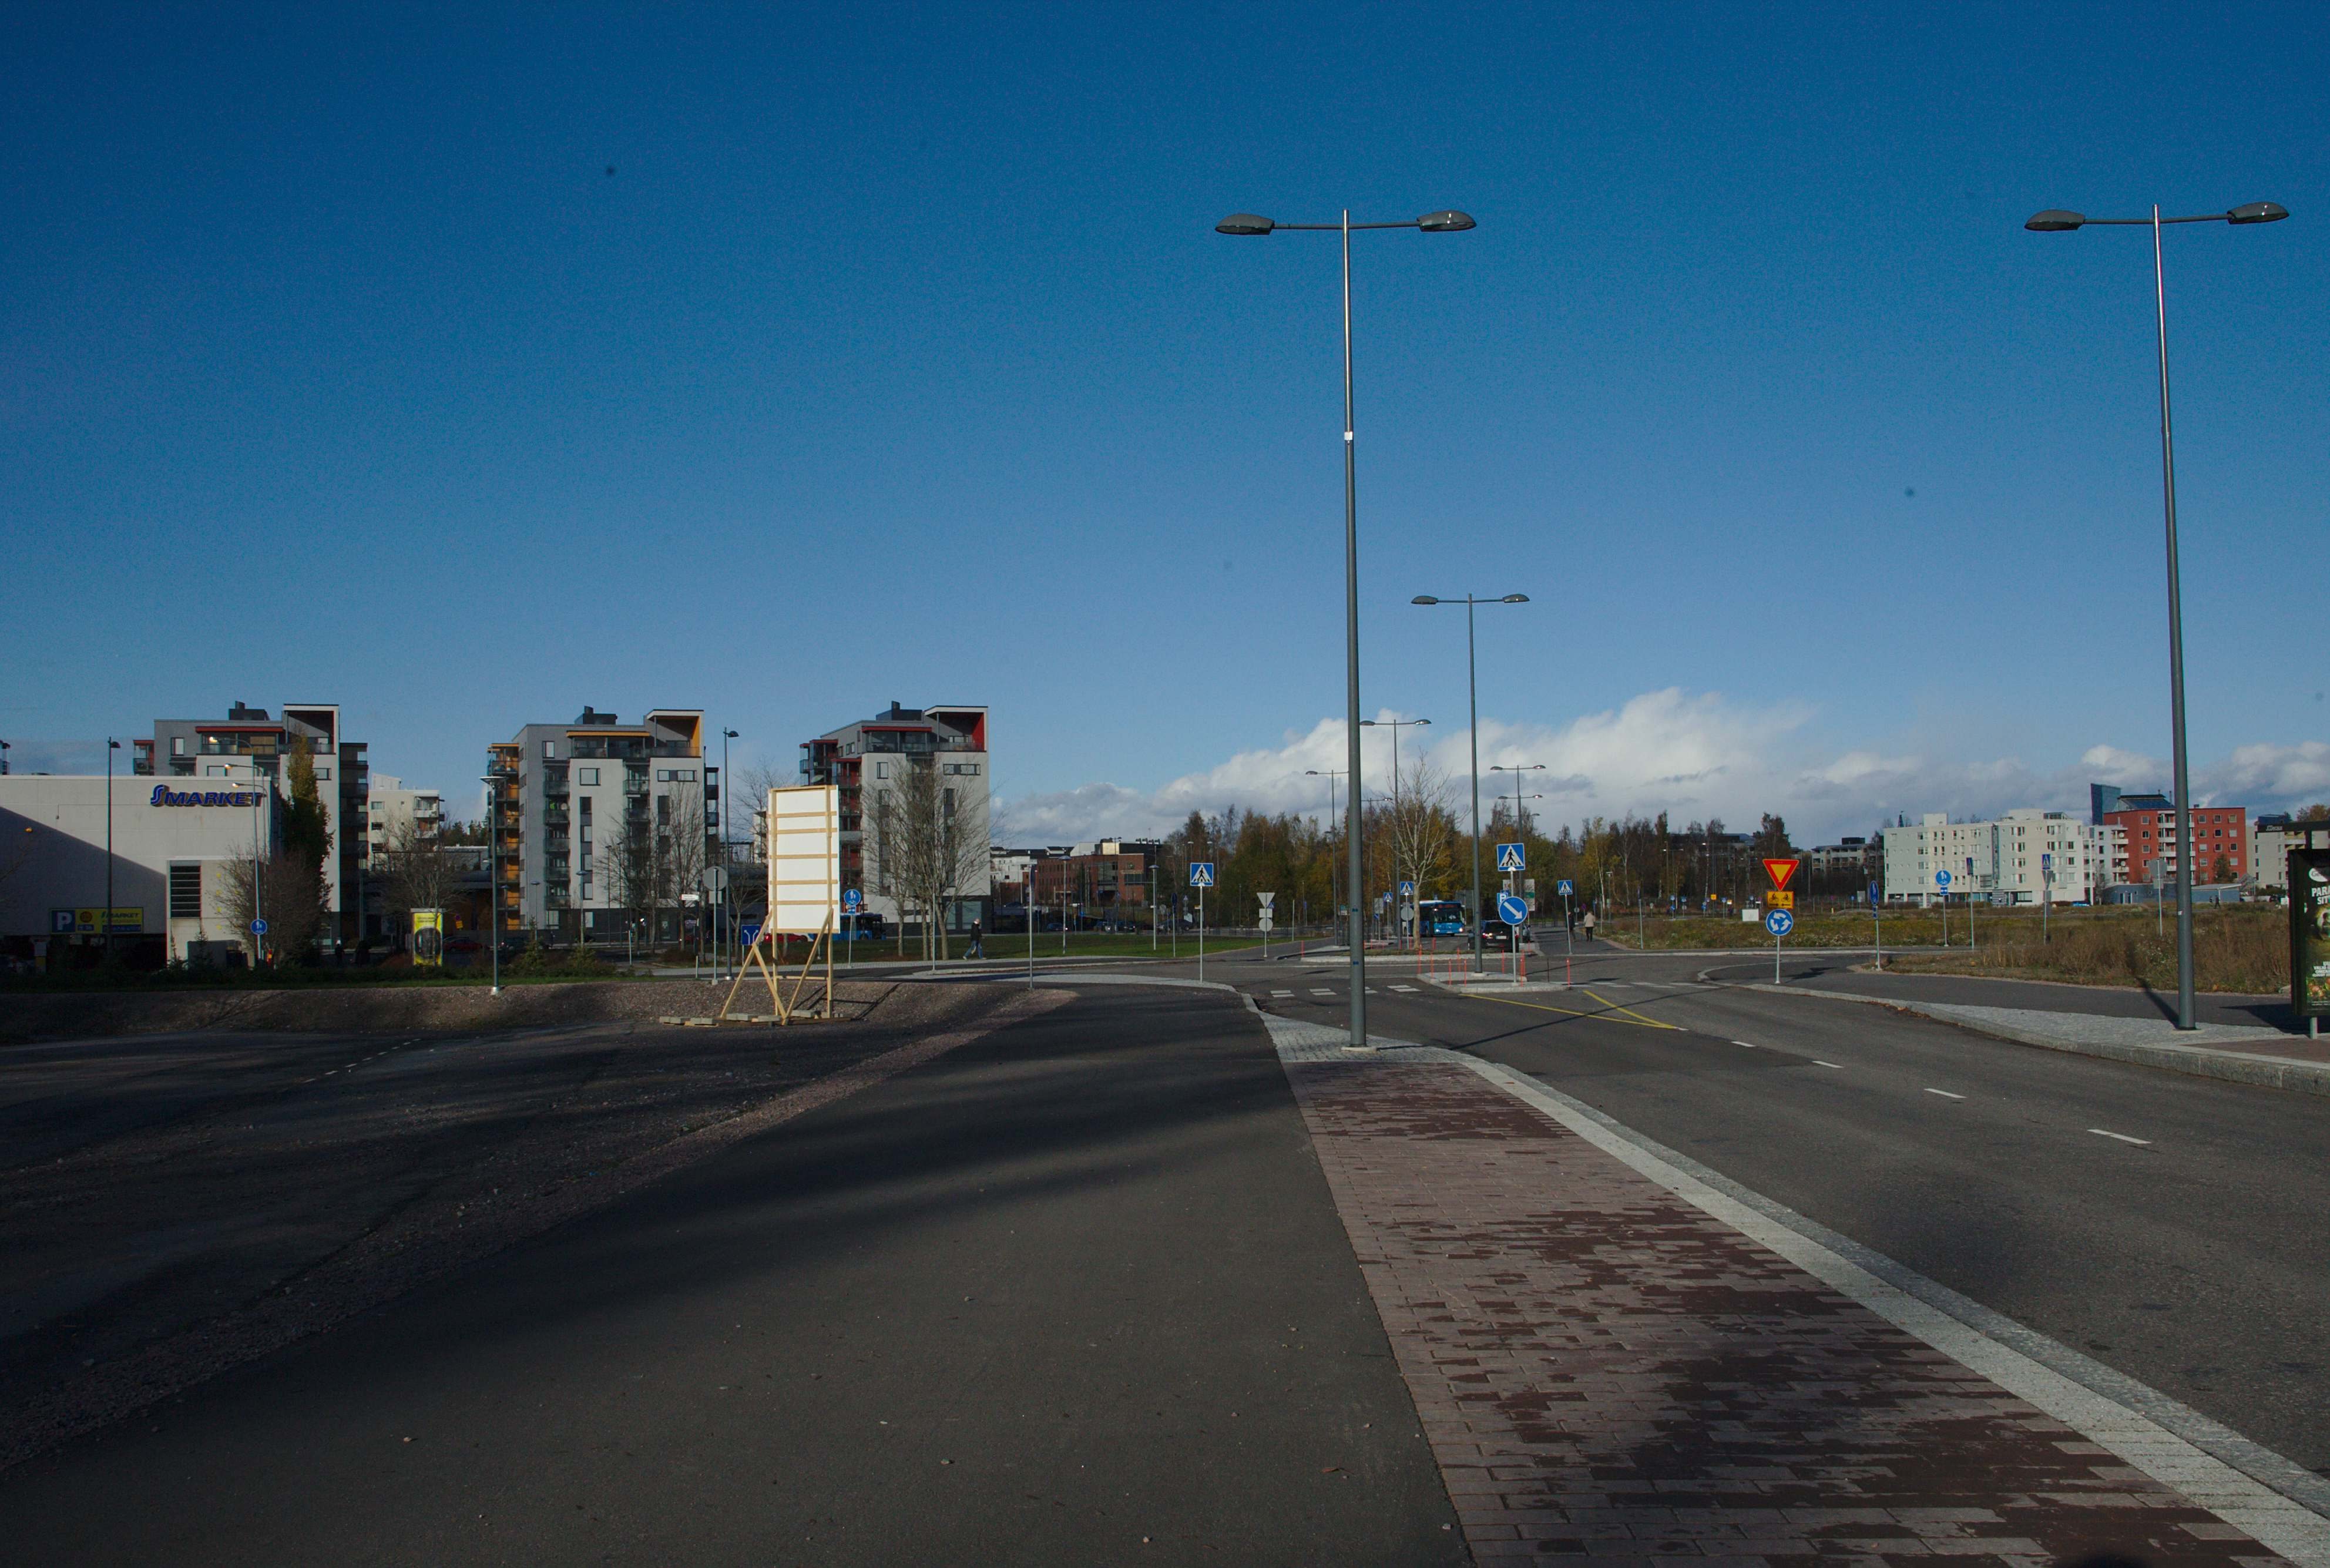
\includegraphics[keepaspectratio,width=.5\textwidth]{modern} & \desc{4cm}{\circledd{2} Example of modern city design in Espoon Keskus (close to railway station)}\\[.2cm]
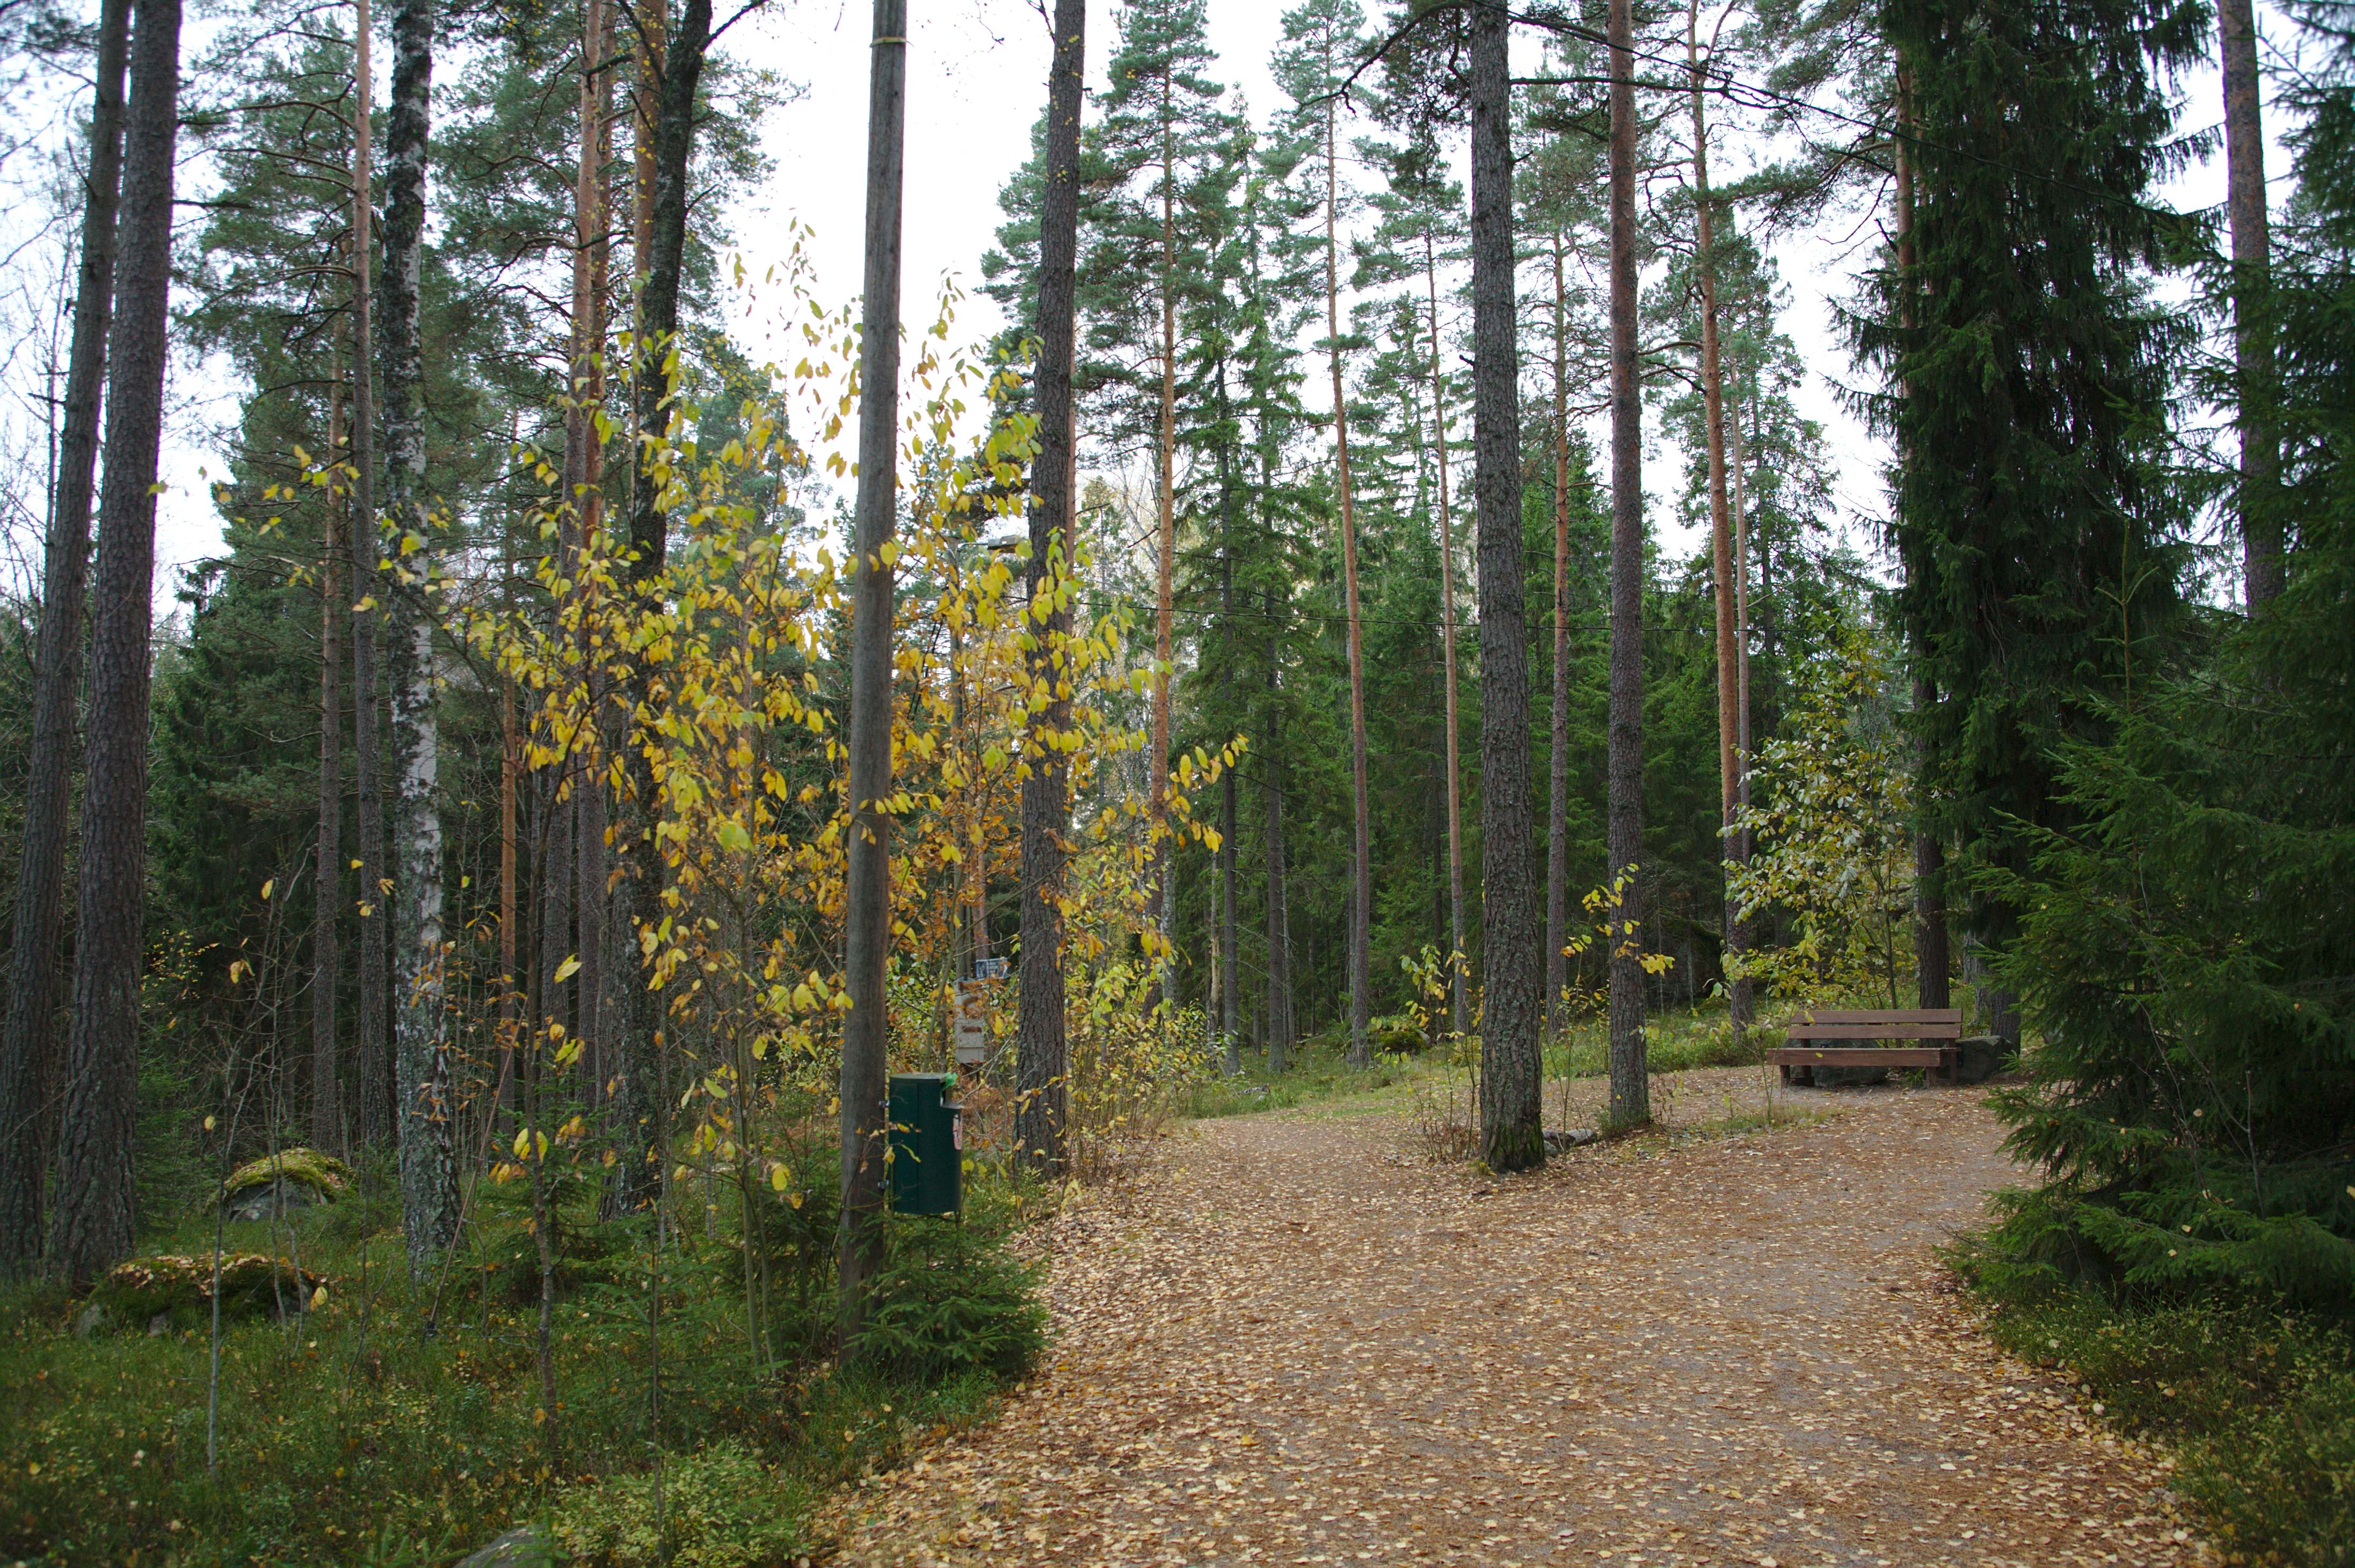
\includegraphics[keepaspectratio,width=.5\textwidth]{green} & \desc{4cm}{\circledd{3} Green city design (Park).}\\
\end{tabular}

\begin{thebibliography}{9}
\bibitem{espoofacts} \myhref{http://www.visitespoo.fi/visitors_guide/espoo-en/public_services}{Espoo in brief. ``Visit Espoo'' web site.}
\bibitem{gov} \myhref{http://www.espoo.fi/en-US/Housing_and_environment/Housing/City_centres}{Espoo city centers. Espoo web cite.}
\bibitem{espoo1855} \myhref{http://www.vanhakartta.fi/historialliset-kartat/kaupunkikartat/sekalaiset-kaupunkikartat/@@mapview?handle=hdl_123456789_6888}{Kalmbergin kartasto R VII : List 7. 1855.}
\bibitem{espoo1945} \myhref{http://koti.kapsi.fi/timomeriluoto/KARTAT/Topografiset\%20kartat/Topografinen\%20kartta\%201:20.000\%20Espoo\%201945.jpg}{Topografinen kartta 1:20.000 Espoo 1945.}
\bibitem{espoo2013} \myhref{http://www.openstreetmap.org/\#map=14/60.2034/24.6415}{OpenStreetMap. Espoo. 2013.}
\bibitem{wikip} \myhref{http://en.wikipedia.org/wiki/Espoo}{Espoo: Wikipedia article.}
\bibitem{keha3} \myhref{http://en.wikipedia.org/wiki/Ring_III}{Ring III: Wikipedia article.}
\end{thebibliography}
\end{document}
